% Created 2018-07-12 Thu 12:39
% Intended LaTeX compiler: pdflatex
\documentclass[11pt]{article}
\usepackage[utf8]{inputenc}
\usepackage{lmodern}
\usepackage[T1]{fontenc}
\usepackage{fixltx2e}
\usepackage{graphicx}
\usepackage{longtable}
\usepackage{float}
\usepackage{wrapfig}
\usepackage{rotating}
\usepackage[normalem]{ulem}
\usepackage{amsmath}
\usepackage{textcomp}
\usepackage{marvosym}
\usepackage{wasysym}
\usepackage{amssymb}
\usepackage{amsmath}
\usepackage[version=3]{mhchem}
\usepackage[numbers,super,sort&compress]{natbib}
\usepackage{natmove}
\usepackage{url}
\usepackage{minted}
\usepackage{underscore}
\usepackage[linktocpage,pdfstartview=FitH,colorlinks,
linkcolor=blue,anchorcolor=blue,
citecolor=blue,filecolor=blue,menucolor=blue,urlcolor=blue]{hyperref}
\usepackage{attachfile}
\author{Myrthe}
\date{\today}
\title{Titanic}
\begin{document}

\tableofcontents





\section{Preface}
\label{sec:orgf83ea19}


\section{Introduction}
\label{sec:org7ed802b}


\begin{equation*}
\label{eq:1}
a^2 + b^2 = c^2
\end{equation*}


\begin{equation}
\label{eq:3}
\delta
\end{equation}


\begin{equation}
\label{eq:2}
\Sigma + \delta \psi = \sum_{i=1}^{N} x_i^2
\end{equation}

\emph{italics}

\textbf{bold}

See equation\footnote\{\label{fn:1}in een voetnoot\}
see equation (\ref{eq:2})



\section{Research}
\label{sec:org25d1bca}

\subsection{python}
\label{sec:org0f46cf4}

lhalkjd 

aldkjfjasd 


\begin{itemize}
\item bullet 1
\item bullet
\item 3
\end{itemize}



aljlaskjd

\begin{minted}[frame=lines,fontsize=\scriptsize,linenos]{ipython}
import matplotlib.pyplot as plt
import numpy as np
%matplotlib inline
\end{minted}

\begin{minted}[frame=lines,fontsize=\scriptsize,linenos]{ipython}
range_x = np.arange(-2,2.1,0.1)
plt.plot(range_x,[x**2 for x in range_x])
plt.show()
\end{minted}

\begin{center}
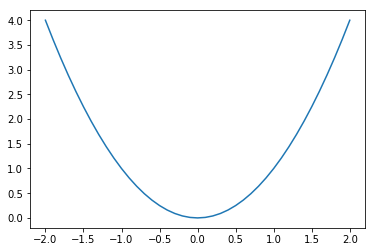
\includegraphics[width=.9\linewidth]{obipy-resources/c7aa849f2540e8b998ec298a9559d3bf-13165Xwa.png}
\end{center}


See footnote \ref{fn:1}
\end{document}